\documentclass[12pt, letterpaper]{article}
\date{\today}
\usepackage[margin=1in]{geometry}
\usepackage{amsmath}
\usepackage{hyperref}
\usepackage{cancel}
\usepackage{amssymb}
\usepackage{fancyhdr}
\usepackage{pgfplots}
\usepackage{booktabs}
\usepackage{pifont}
\usepackage{amsthm,latexsym,amsfonts,graphicx,epsfig,comment}
\pgfplotsset{compat=1.16}
\usepackage{xcolor}
\usepackage{tikz}
\usetikzlibrary{shapes.geometric}
\usetikzlibrary{arrows.meta,arrows}
\newcommand{\Z}{\mathbb{Z}}
\newcommand{\N}{\mathbb{N}}
\newcommand{\R}{\mathbb{R}}
\newcommand{\Po}{\mathcal{P}}

\author{Alex Valentino}
\title{Homework }
\pagestyle{fancy}
\renewcommand{\headrulewidth}{0pt}
\renewcommand{\footrulewidth}{0pt}
\fancyhf{}
\rhead{
	Challange Problem Set 1 \\
	292	
}
\lhead{
	Alex Valentino\\
}
\begin{document}
	\begin{enumerate}
		\item 
		\begin{itemize}
			\item Show that $x(t)$ satisifes $\| A^{-1} x(t)\|^2 = 1$.
			\begin{align*}
				\| A^{-1} x(t)\|^2 &= \| A^{-1} A u(t)\|^2\\
				&= \| u(t)\|^2\\
				&= \| \begin{bmatrix}
				\cos(t)\\
				\sin(t)
				\end{bmatrix}\|^2\\
				&= \cos^2(t) + \sin^2(t)\\
				&= 1.
			\end{align*}
			\item Show that the equation above may be written as $x \cdot M x = 1$.
			\begin{align*}
				x \cdot M x &= x^T M x\\
				&= x^T (A^{-1})^T A^{-1} x\\
				&= (A^{-1}x)^T A^{-1}x\\
				&= A^{-1}x \cdot A^{-1}x\\
				&= \|A^{-1}x\|^2 \\
				&= 1.
			\end{align*}
			\item Show that $M$ is symmetric.
			\begin{align*}
			M^T &= ((A^{-1})^T A^{-1})^T\\
			&= (A^{-1})^T ((A^{-1})^T)^T\\
			&= (A^{-1})^T A^{-1}\\
			&= M
			\end{align*}
			\item Suppose $M = \begin{bmatrix}
			a & c \\ c & b
\end{bmatrix}			 $.  We must show that $x \cdot M x$ can be written as $ax^2 + by^2 + 2cxy$.
			\begin{align*}
				1 &= x \cdot M x\\
				&= \begin{bmatrix}
				x & y
				\end{bmatrix}\begin{bmatrix}
			a & c \\ c & b
\end{bmatrix}\begin{bmatrix}
				x \\ y
				\end{bmatrix}\\
				&= \begin{bmatrix}
				x & y
				\end{bmatrix}\begin{bmatrix}
			ax + cy \\ cx + by
\end{bmatrix}\\
	&= ax^2 + by^2 + 2cxy.
			\end{align*}
		\end{itemize}
		\item 
		\begin{itemize}
			\item Show that both $\lambda_1$ and $\lambda_2$ are positive.  Since $x \cdot M x = \|A^{-1}x\|^2$, then all outputs of $x \cdot M x$ are strictly positive.  Suppose $x = u_1$, then $u_1 \cdot M u_1 = u_1 \cdot \lambda_1 u_1 = \lambda_1 \|u_1\|^2 = \lambda_1 > 0$.  A similar proof exists for $u_2$.  Therefore the eigenvalues are strictly positive.   
			\item Suppose $\lambda_1 = \lambda_2$.  We must show that $\| x(t) \| = \frac{1}{\sqrt{\lambda_1}}$.  Let $U$ be the matrix where $u_1$ and $u_2$ are columns.  Since $u_1, u_2$ are orthonormal, then $U$ is an orthogonal matrix.  Therefore $U^{-1} = U^T$.  Let $D = \begin{bmatrix}
			\lambda_1 & 0\\
			0 & \lambda_2\\
\end{bmatrix}			 $, and let $q = \begin{bmatrix}
q_1(t)\\q_2(t)
\end{bmatrix} = U^T x$.  Since $M$ is diagonalizable we may rewrite $x \cdot M x$ as follows: 
			$$
				1 = x \cdot M x = x \cdot UMU^T x = q^T U^T UMU^T Uq = q \cdot D q = \lambda_1 q_1^2(t) + \lambda_2 q_2^2(t).  			
			$$
			This equation defines an ellipse paramaterized by $q_1(t) = \pm \frac{1}{\sqrt{\lambda_1}}\cos(t), q_2(t) = \pm \frac{1}{\sqrt{\lambda_2}}\sin(t)$.  Since $q = U^T x$, then $x=Uq$, therefore we may explicitly solve for $x$ via $x = Uq = \pm (\frac{1}{\lambda_1}\cos(t)u_1 + \frac{1}{\lambda_2}\sin(t)u_2)$.  Therefore if $\lambda_1 = \lambda_2$, then $\|x\| = \sqrt{\frac{\cos^2(t)}{\lambda_1} + \frac{\sin^2(t)}{\lambda_2} } = \sqrt{\frac{\cos^2(t)}{\lambda_1} + \frac{\sin^2(t)}{\lambda_1} } = \frac{1}{\sqrt{\lambda_1}}$.
			\item Consider the case where $\lambda_1 > \lambda_2$.  Note that $\|x\|^2 =\frac{\cos^2(t)}{\lambda_1} + \frac{\sin^2(t)}{\lambda_2} = u \cdot \begin{bmatrix}
			\frac{1}{{\lambda_1}} &0\\ 0 & \frac{1}{{\lambda_2}}
\end{bmatrix}u			 $, let the matrix in the quadratic function above be denoted $S^2$.  By lemma 19 in the previous carlen multivarible textbook, $ \|x\|^2$ on the unit circle is maximized and minimized by the eigenvalues of $S^2$.  For the matrix $S^2$ the eigenvalues are obviously $\frac{1}{\lambda_1}, \frac{1}{\lambda_2}$.  Since $\lambda_1 > \lambda_2$, then $\frac{1}{\lambda_1} < \frac{1}{\lambda_2}$, therefore making $\frac{1}{\lambda_2}$ the maximum of $\|x\|^2$, and therefore forcing $\frac{1}{\lambda_1}$ to be the minimum.  Since $\sqrt{}$ is a monotonically increasing function on $\R_+$, then $\|x\|$ has a maximum of $\frac{1}{\sqrt{\lambda_2}}$ and a minimum of $\frac{1}{\sqrt{\lambda_1}}$.  We must show that $\|x\|$ is maximal if and only if $x(t) = \pm \frac{1}{\lambda_2}u_2$.
			\begin{itemize}
				\item Suppose $x(t) = \pm \frac{1}{\lambda_2} u_2$.  We must show that $\|x(t)\|$ is maximal.  
				$$
				\|x(t)\| = \sqrt{\frac{\cos^2(t)}{\lambda_1} + \frac{\sin^2(t)}{\lambda_2} } \leq  \sqrt{\frac{\cos^2(t)}{\lambda_2} + \frac{\sin^2(t)}{\lambda_2} } = \frac{1}{\sqrt{\lambda_2}} = \|\pm \frac{1}{\sqrt{\lambda_2}} u_2\|			
				$$
				\item Suppose $\|x(t)\|$ is maximal.  We must show that $x(t) = \pm \frac{1}{\sqrt{\lambda_2}} u_2$.  Since $\|x(t)\|$ is maximal and $\|x(t)\|$ has a single maximum then $\|x(t)\| = \frac{1}{\sqrt{\lambda_2}}$.  Therefore:
				\begin{align*}
				\|x(t)\|^2 &= \frac{1}{\lambda_2}\\
				\frac{\cos^2(t)}{\lambda_1} + \frac{\sin^2(t)}{\lambda_2} &= \frac{1}{\lambda_2}\\
				\frac{\cos^2(t)}{\lambda_1} &= \frac{1}{\lambda_2}(1-\sin^2(t))\\
				\frac{\cos^2(t)}{\lambda_1} &= \frac{\cos^2(t)}{\lambda_2}\\
				\cos^2(t)(\frac{1}{\lambda_1}-\frac{1}{\lambda_2}) &= 0.
				\end{align*}  Since $\lambda_1 > \lambda_2$, then the only solution to that equation is when $\cos^2(t) = 0$, thus when $\cos(t) = 0$.  Therefore evaluating $x(t)$ when $cos(t) = 0$ yields $x(t) = \pm (\frac{1}{\lambda_1}\cos(t)u_1 + \frac{1}{\lambda_2}\sin(t)u_2) = \pm \frac{1}{\lambda_2}\sin(t)u_2 = \pm \frac{1}{\lambda_2}\sqrt{1-\cos^2(t)}u_2 = \pm \frac{1}{\lambda_2} u_2$.  
		The proof for $x(t) = \pm \frac{1}{\lambda_1} u_1$ if and only if $\|x(t)\|$ is minimal is nearly identical to the one above, simply replace maximal with minimal, finding $\sin(t) = 0$, changing the direction of an inequality with substituting $\lambda_2$ for $\lambda_1$.  
\iffalse				
				$x^2$ is strictly increasing on $\R_+$ then $\|x(t)\|^2$ is maximal.  This is equivalent to $\begin{bmatrix}
			\frac{1}{\lambda_1} & 0\\ 0 & \frac{1}{\lambda_2}	
\end{bmatrix}				 $
\fi
			\end{itemize}
		\end{itemize}
		\item Let $$v_1 = \frac{1}{\sqrt{\lambda_1}} A^{-1}u_1, v_2 = \frac{1}{\sqrt{\lambda_2}} A^{-1}u_2.$$
		\begin{itemize}
			\item Show that $\{v_1, v_2\}$ is an orthonormal basis for $\R^2$.  By definition of orthonormal basis we must show that $v_1 \cdot v_2 = 0, v_1 \cdot v_1 = v_2 \cdot v_2 = 1.$
			\begin{itemize}
				\item \begin{align*}
					v_1 \cdot v_2 &= v_1^T v_2\\
					&= \frac{1}{\sqrt{\lambda_1}} (A^{-1}u_1)^T \frac{1}{\sqrt{\lambda_2}} A^{-1}u_2\\
					&= \frac{1}{\sqrt{\lambda_1 \lambda_2}} u_1^T (A^{-1})^TA^{-1} u_2\\
					&= \frac{1}{\sqrt{\lambda_1 \lambda_2}} \lambda_2 u_1^T u_2\\
					&= 0
				\end{align*}
				\item Let $i \in \{1,2\}$ \begin{align*}
					v_i \cdot v_i &= v_i^T v_i\\
					&=  \frac{1}{\sqrt{\lambda_i}} (A^{-1}u_i)^T \frac{1}{\sqrt{\lambda_i}} A^{-1}u_i\\
					&= \frac{1}{\lambda_i}u_i^T (A^{-1})^T A^{-1} u_i\\
					&= \frac{1}{\lambda_i} u_i^T M u_i\\
					&= \frac{\lambda_i}{\lambda_i} u_i^T u_i\\
					&= 1.
				\end{align*} 
			\end{itemize}
			\item We must show that $\|x(t)\|$ is maximal if and only if $(\cos(t), \sin(t)) = \pm v_2$.
			\begin{itemize}
				\item Suppose $\|x(t)\|$ is maximal.  We must show that $(\cos(t), \sin(t)) = \pm v_2$.  We know from exercise 3 that $x(t) = \pm \frac{1}{\sqrt{\lambda_2}} u_2$.  Therefore 
				\begin{align*}
				x(t) &= \pm \frac{1}{\lambda_2} u_2\\
				A(\cos(t),\sin(t)) &= \pm \frac{1}{\sqrt{\lambda_2}} u_2\\
				(\cos(t),\sin(t)) &= \pm \frac{1}{\sqrt{\lambda_2}} A^{-1} u_2\\
				(\cos(t),\sin(t)) &= \pm v_2.
				\end{align*}
				\item Suppose $(\cos(t), \sin(t)) = \pm v_2$.  We must show that $\|x(t)\|$ is maximal.  
				Therefore 
				$$
				x(t) = A(\cos(t), \sin(t)) = \pm A v_2 = \pm \frac{1}{\sqrt{\lambda_2}} A A^{-1} u_2 = \pm \frac{1}{\sqrt{\lambda_2}} u_2.
				$$
				
				Thus by exercise 3 since $x(t) = \pm \frac{1}{\sqrt{\lambda_2}} u_2$ then $\|x(t)\|$ is maximal.  
			\end{itemize}
		\end{itemize}
		The proof is identical for showing $\|x(t)\|$ is minimal if and only if $(\cos(t), \sin(t)) = \pm v_1$ by swapping $2$ for $1$ and using the minimal portion of what was proved in exercise 3.
		\item Let $A = \begin{bmatrix}
 1 & 0 \\
 1 & \sqrt{3} \\
\end{bmatrix}		 $. Let $M = (A^{-1})^T A^{-1}$ This has the corresponding characteristic polynomial of $(\lambda - \frac{1}{6} (5-\sqrt{13}))(\lambda - \frac{1}{6} (5+\sqrt{13})) = 0$, thus the eigenvalues $\mu_1 = \frac{1}{6} (5+\sqrt{13}), \mu_2 = \frac{1}{6} (5-\sqrt{13})$  Therefore $\sigma_1 = \sqrt{\frac{6}{5+\sqrt{13}}}, \sigma_2 = \sqrt{\frac{6}{5-\sqrt{13}}}$.  This gives us the major axis of length of $\sigma_2 = 2.07431$ and the minor axis length of $\sigma_1 = 0.835$.  These correspond to $u_1 = (0.957092, 0.289784)$ and $u_2 = (0.289784, -0.957092)$.  The angle between $u_1$ and the x-axis is $0.294001$ radians.
	The ellipse looks like: 
	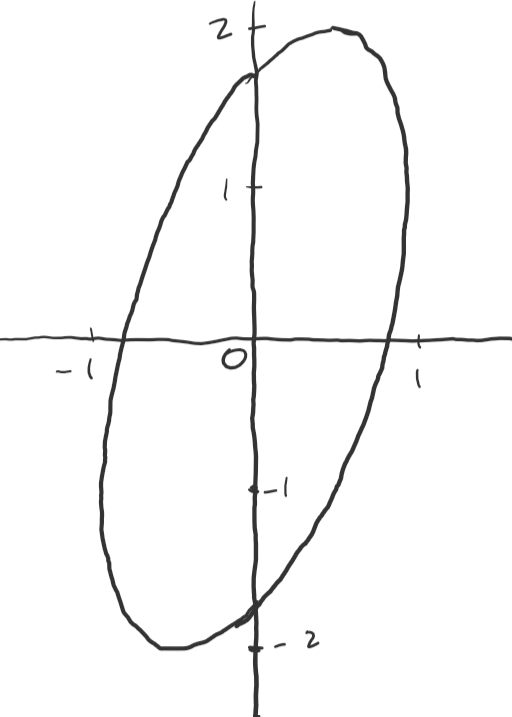
\includegraphics[scale=1.0]{challangeProblemSet1-292-ellipse.png}  
	\item Let $V = \begin{bmatrix}
	v_1 & v_2
\end{bmatrix}	, S = \begin{bmatrix}
\sigma_1 & 0\\ 0& \sigma_2
\end{bmatrix}, U = \begin{bmatrix}
u_1 & u_2
\end{bmatrix} $  We must show that $\sigma_1 (x\cdot v_1)u_1 + \sigma_2 (x\cdot v_2)u_2 = USV^T x$.  Therefore
\begin{align*}
	\sigma_1 (x\cdot v_1)u_1 + \sigma_2 (x\cdot v_2)u_2 &= U(\sigma_1 (x\cdot v_1), \sigma_2 (x\cdot v_2))\\
	&= US(v_1 \cdot x, v_2 \cdot x)\\
	&= USV^T x
\end{align*}
	Therefore $A = USV^T$.
	\item Let $A = \begin{bmatrix}
	11 & -5\\2 & -10
\end{bmatrix}$  We must find orthogonal matrices $U,V$ and diagonal matrix $S$ such that $A = USV^T$.  Note that $A^T A$ has eigenvalues of  $200$ and 50 and these correspond with the eigenvectors $(\frac{-1}{\sqrt{2}},\frac{1}{\sqrt{2}})$ and $(\frac{1}{\sqrt{2}},\frac{1}{\sqrt{2}})$.  Since $A^T A = V S^2 V^T$ then $S = \begin{bmatrix}
10\sqrt{2} & 0 \\ 0 & 5\sqrt{2}
\end{bmatrix}, V = \begin{bmatrix}
\frac{-1}{\sqrt{2}} & \frac{1}{\sqrt{2}}\\
\frac{1}{\sqrt{2}} & \frac{1}{\sqrt{2}}
\end{bmatrix}$. Note that $A A^T$ has eigenvectors of           $(\frac{3}{5}, -\frac{4}{5})$ and $(-\frac{4}{5},-\frac{3}{5})$ and corresponding to the same eigenvalues of $50$ and $200$.  Note that $A A^T = U S^2 U^T$, thus we have found $U = \begin{bmatrix}
-\frac{4}{5} & \frac{3}{5}\\
-\frac{3}{5} & -\frac{4}{5}
\end{bmatrix} $.  
	Verification:
		\begin{align*}
			USV^T &=  \begin{bmatrix}
-\frac{4}{5} & \frac{3}{5}\\
-\frac{3}{5} & -\frac{4}{5}
\end{bmatrix} \begin{bmatrix}
10\sqrt{2} & 0 \\ 0 & 5\sqrt{2}
\end{bmatrix} \begin{bmatrix}
\frac{-1}{\sqrt{2}} & \frac{1}{\sqrt{2}}\\
\frac{1}{\sqrt{2}} & \frac{1}{\sqrt{2}}
\end{bmatrix}\\
&=\begin{bmatrix}
-\frac{4}{5} & \frac{3}{5}\\
-\frac{3}{5} & -\frac{4}{5}
\end{bmatrix} \begin{bmatrix}
-10 & 10 \\
 5 & 5 
\end{bmatrix}\\
&= \begin{bmatrix}
11 & -5 \\
 2 & -10 
\end{bmatrix}\\
&= A.
		\end{align*}
	\end{enumerate}
\end{document}